\documentclass[border=10pt]{standalone}
\usepackage{pgfplots}
\usepgfplotslibrary{colormaps}
\pgfplotsset{trig format plots=rad}
\begin{document}
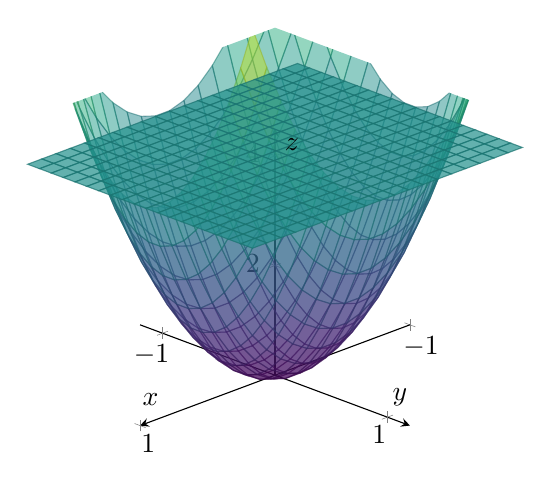
\begin{tikzpicture}
\begin{axis}[
    view={135}{30},
    xlabel=$x$, ylabel=$y$, zlabel=$z$,
    axis lines=center,
    grid=both,
    colormap/viridis,
    samples=20,
    domain=-1.2:1.2,
    ymin=-1.2, ymax=1.2,
    zmin=0, zmax=4.5,
]
    % We plot z = 4(x^2 + y^2) to represent the paraboloid
    % This is the same shape as x = 4(y^2 + z^2) but oriented differently
    \addplot3[surf, opacity=0.5, domain=-1:1, y domain=-1:1] {4*(x^2 + y^2)};
    
    % Cap at z = 4
    \addplot3[surf, opacity=0.7, domain=-1:1, y domain=-1:1] {4};

\end{axis}
\end{tikzpicture}
\end{document}
